\begin{figure*}[t!]
\centering
\tikzset{%
process/.style  = {rectangle, minimum width=1cm, minimum height=1cm, align=flush center, draw=black, inner sep=0.2cm},
decision/.style = {diamond, minimum width=1cm, minimum height=1cm, align=flush center, draw=black, inner sep=0cm},
resource/.style = {shape=rounded rectangle, minimum width=1cm, minimum height=1cm, align=flush center, draw=black},
stop/.style     = {rectangle, minimum width=1cm, minimum height=1cm, align=flush center, draw=black, double, thick},
waypoint/.style = {coordinate}
}
\newcommand{\cbox}[2]{\parbox{#1}{\centering
#2}}
\newcommand{\mrule}[1]{\rule[0.8ex]{#1}{0.4pt}}
\resizebox{0.85\textwidth}{!}{%
\begin{tikzpicture}[
thick,
>/.tip=Latex,
loose/.style={inner sep 0.7em}]
\draw
	node at (0,0) [font=\large] (statement) {input: If $\langle$\textState$\rangle$ then $\langle$\textAction$\rangle$ because $\langle$\textGoal$\rangle$}
	
	node [process, below of=statement, node distance=1.5cm, left=0.1cm, fill=gray(x11gray)] (parse) {\cbox{3.5cm}{Parse Statement: \\
	$\begin{array}{lcr} \state \leftarrow \text{\textState} \\ 
	\action \leftarrow \text{\textAction} \\
	\goal \leftarrow \text{\textGoal} \end{array}$}}
	
    node [decision,right of=parse,node distance=4cm, fill=lavendergray] (in_k) {\cbox{1.5cm}{Is $G$ in \KB?}}
    
    node [decision,below of=in_k,node distance=2.1cm,minimum width=1.5cm, fill=lavendergray] (loop) {$i>n$?}
    
    node [process,below of=loop,node distance=2.6cm, fill=magnolia] (startFeedback) {\parbox{3.5cm}{Ask the user for more\\ information $G'(Z)$. \\\mrule{3.5cm} \\ $i=i+1$ \\ $\mathrm{goalStack}.push(\goal)$ \\ $ \goal = G' (Z)$}}
    
        node[waypoint,left of=startFeedback,node distance=2.9cm] (loop_0) {}
        node[waypoint,above of=loop_0,node distance=2.5cm] (loop_1) {}
        node[waypoint,above of=loop_1,node distance=2.2cm, right=1.7cm] (loop_2) {}
    
    node[stop,left of=loop,node distance=1.75cm,fill=pearl] (fail0) {Fail}
    
    %%
    node[decision,right of=in_k,node distance=4.5cm,minimum width=3cm, fill=lavendergray] (empty) {\cbox{1.5cm}{goalStack empty?}}
    
    node[process, right of=empty, node distance=4.5cm, minimum width=2cm, fill=lavenderblush] (prover) {\parbox{3cm}{Neuro-Symbolic \\ Theorem Prover: \\ Prove $\goal$}}
    
    node[process,below of=empty,node distance=3cm,label=below:\emph{knowledge base update loop}, fill=magnolia] (add) {\parbox{4cm}{Add a new rule to \KB \\ \mrule{3cm} \\ $\mathrm{goalStack}.top() \vdash \goal$ \\ $\goal = \mathrm{goalStack}.pop()$}}
    
        node[waypoint,left of=add,node distance=2.7cm] (empty_0) {}
        node[waypoint,above of=empty_0,node distance=3cm] (empty_1) {}
        % node[waypoint,left of=empty_1,node distance=8cm] (empty_2) {}
    
    node[decision,right of=prover,node distance=4cm,minimum width=3.5cm, fill=lavendergray] (prove) {\cbox{1.5cm}{Is there a proof for $\goal$?}}
    
    node[waypoint, below of=prove, node distance=3cm] (empty_2) {}
    
    node[process, below of=prove, right=0.6cm, node distance=3cm, fill=magnolia] (discard) {\parbox{3.5cm}{discard the rules added in the \emph{knowledge base update loop}}}
    
    node[resource,below of=prover,node distance=2cm, fill=lavenderblush] (embeddings0) {\cbox{3cm}{\textcolor{black}{Rule and Variable embeddings}}}
    
    node[stop,below of=discard,node distance=2cm, fill=pearl] (fail1) {Fail}

    node[decision,right of=prove,node distance=5cm,minimum width=5cm,inner sep=-0.2cm, fill=lavendergray] (check_proof) {\cbox{2.2cm}{Does the \\
    proof contain \\
    $\state$ and $\action$? }}
    
    node[waypoint, below of=check_proof, node distance=3cm] (empty_3) {}
    
    % node[stop,below of=check_proof,node distance=4cm, fill=pearl] (fail2) {Fail}
    
    node[stop,right of=check_proof,node distance=4cm,label=below:\emph{proof},fill=pearl] (success) {Succeed};
    
\draw(statement) edge [->] (parse);
\draw(parse) edge [->] (in_k);
%%
\draw(in_k) edge ["Y"',pos=0.05,->] (empty);
\draw(in_k) edge ["N",very near start,->] (loop);
%%
\draw(loop) edge ["Y"',->] (fail0);
\draw(loop) edge ["N",very near start,->] (startFeedback);

    \draw(startFeedback) edge (loop_0);
    \draw(loop_0) edge ["\emph{user feedback loop}"] (loop_1);
    % \draw(loop_1) edge ["\textcolor{brickred}{user feedback loop}", ->] (loop_2);
    \draw(loop_1) edge [->] (loop_2);
%%
\draw(empty) edge ["Y"',->] (prover);
\draw(empty) edge ["N",near start,->] (add);
\draw(prover) edge [->] (prove);

    \draw(add) edge (empty_0);
    \draw(empty_0) edge [->] (empty_1);
    % \draw(empty_1) edge ["\textcolor{brickred}{updating the knowledge base}",->] (empty_2);
%%
\draw(prove) edge ["Y"',->] (check_proof);
\draw(prove) edge ["N",very near start,-] (empty_2);
\draw(empty_2) edge [->] (discard);
\draw(discard) edge [->] (fail1);
\draw(prover) edge [dotted] (embeddings0);
%%
% \draw(check_proof) edge ["Y"',"\textcolor{brickred}{returns proof, i.e. chain of reasoning}",->] (success);
\draw(check_proof) edge ["Y"',->] (success);
\draw(check_proof) edge ["N",near start,-]  (empty_3);
\draw(empty_3) edge [->] (discard);
%%
\end{tikzpicture}
    }%
    
    % 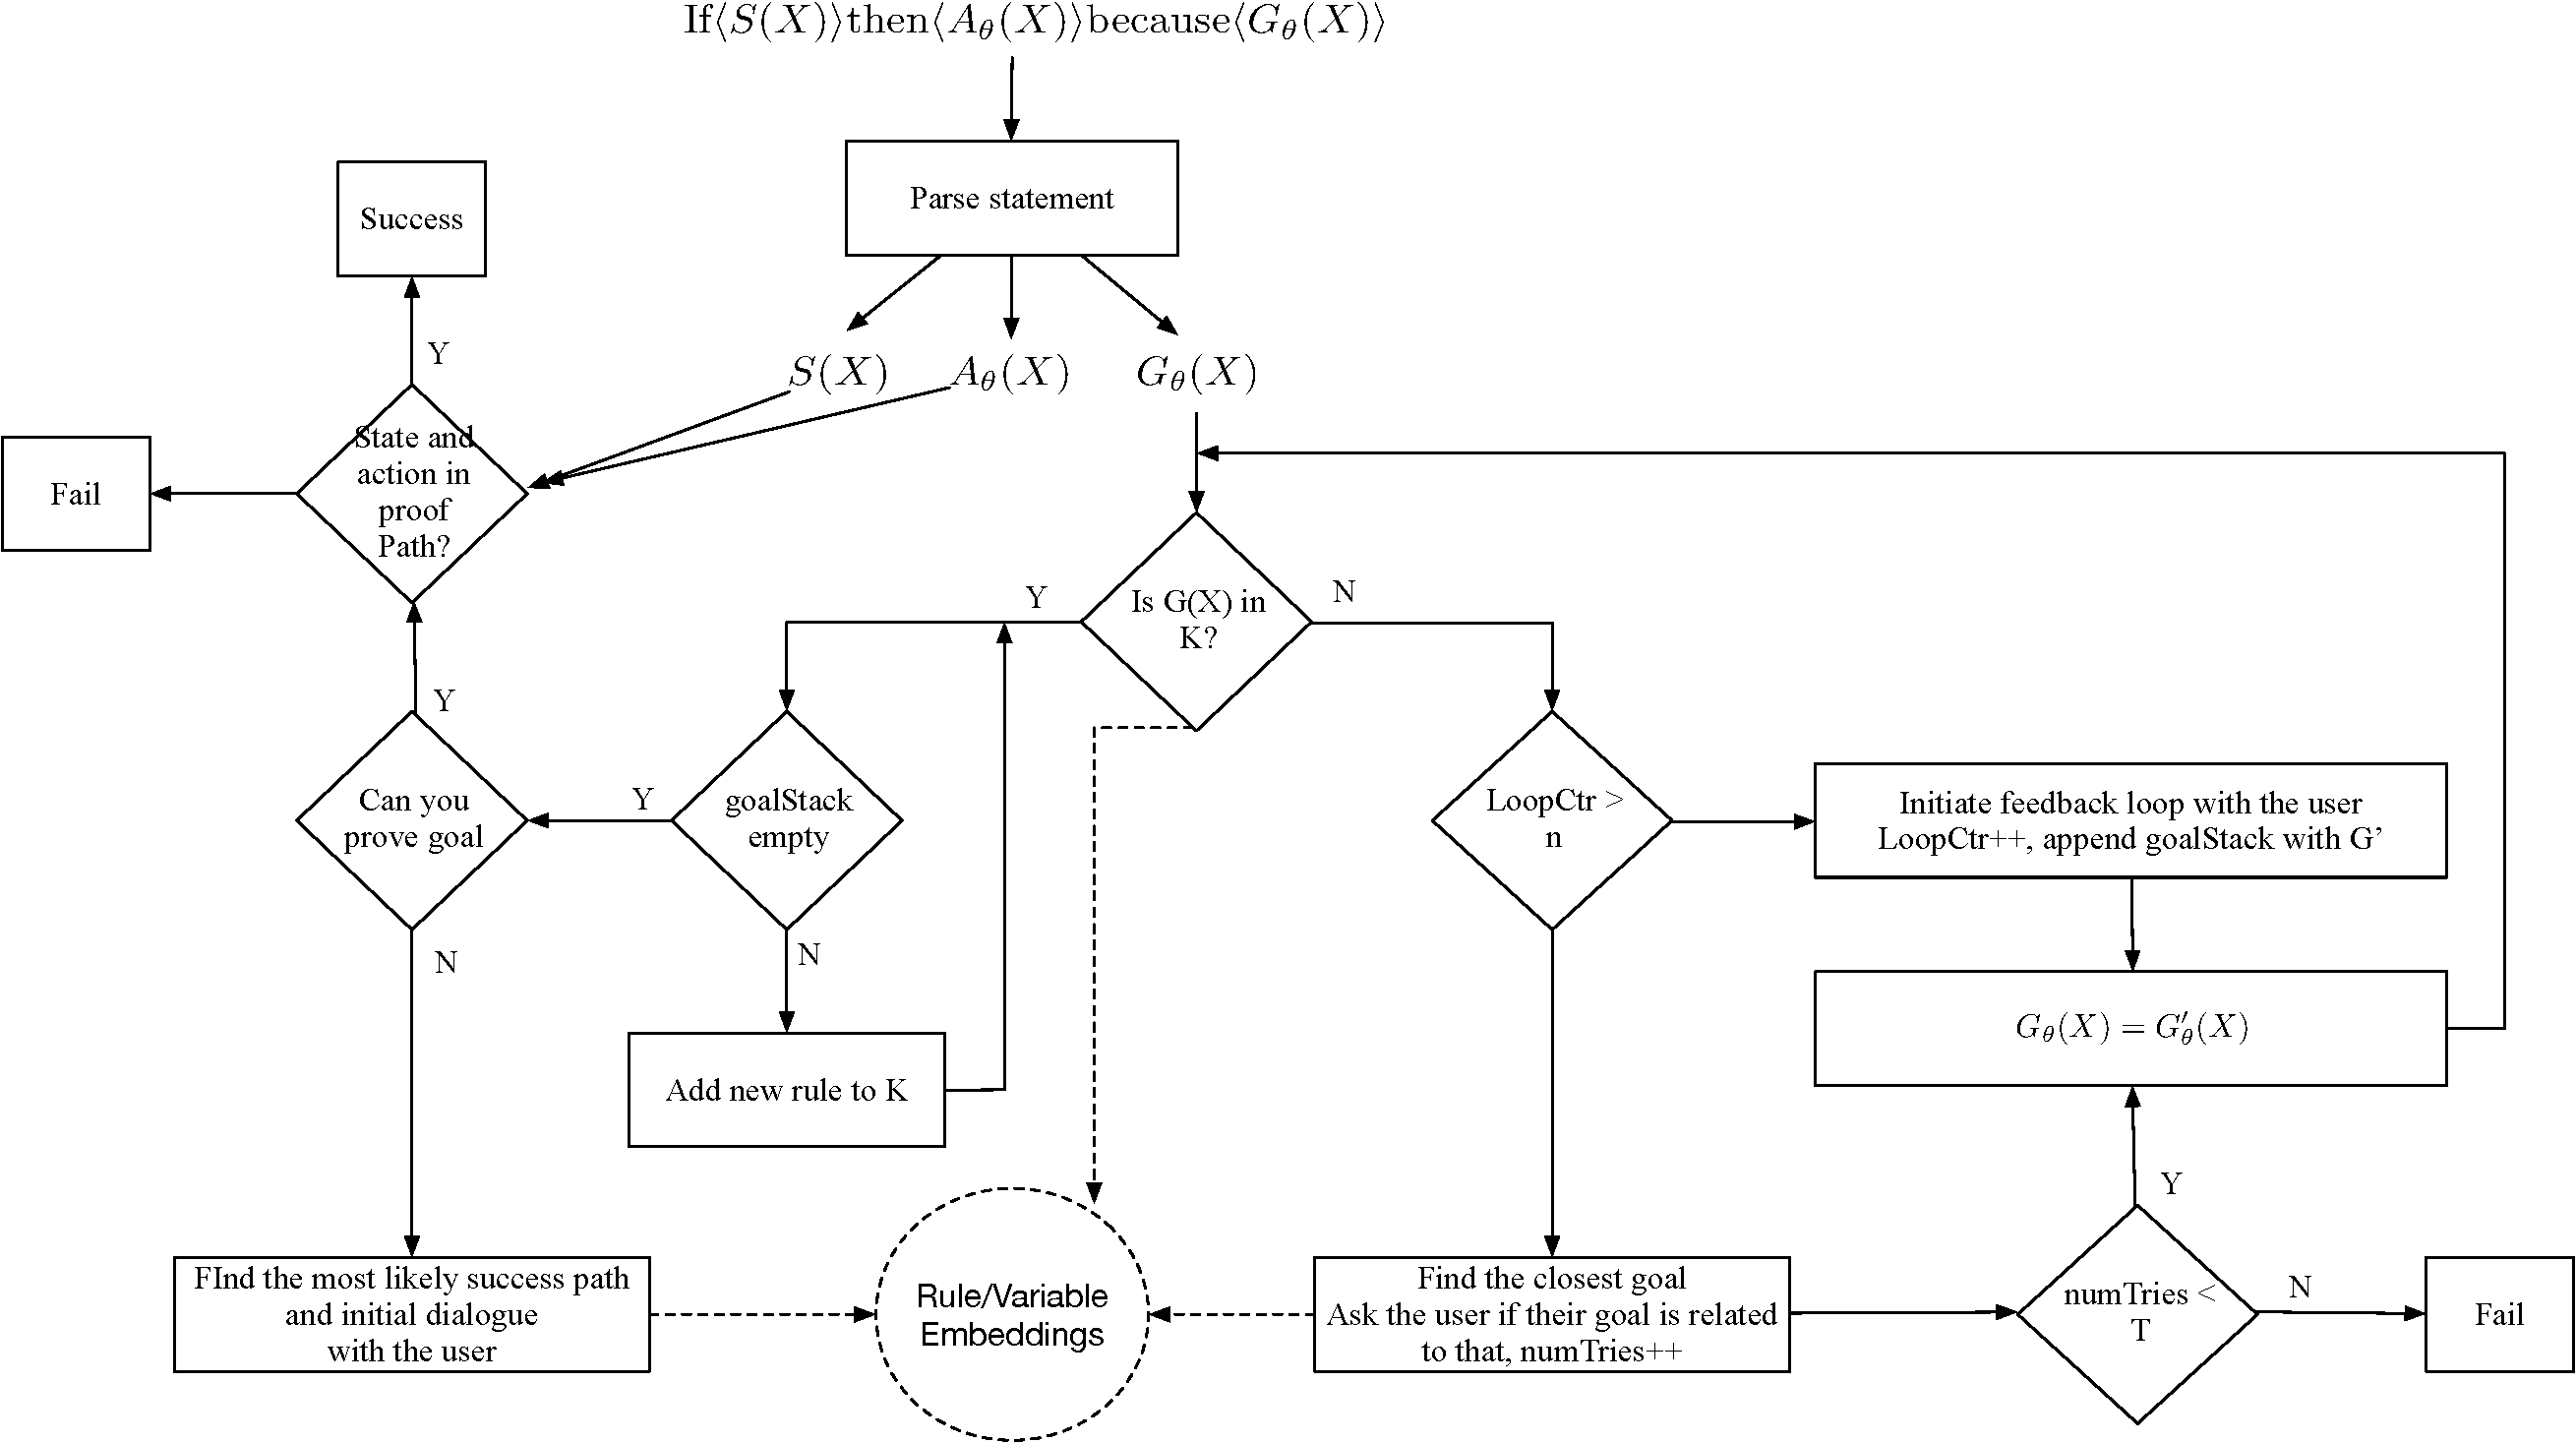
\includegraphics[width=\textwidth]{figs/model.pdf}
    % \caption{Model Architecture \amoscomment{Why 'proposed'? The arrows from S(X) and A(X) make it hard to understand the flow (that is, what happens first, what next). Maybe just remove them or mark it differently (not using arrows).} \facomment{figure is being re-generated}}
    \caption{CORGI's flowchart. The input is an if-then-because command e.g., ``if it snows tonight then wake me up early because I want to get to work on time''. The input is parsed into its logical form representation (for this example, $\state$ = \prologTerm{weather(snow, Precipitation)}). If CORGI succeeds, it outputs a proof tree for the because-clause or \textGoal (parsed into $\goal$=\prologTerm{get(i,work,on$\_$time)}). The output proof tree contains commonsense presumptions for the input statement (Fig \ref{fig:prooftree} shows an example). If the predicate $G$ does not exist in the knowledge base, \KB, (Is $G$ in \KB?), we have missing knowledge and cannot find a proof. Therefore, we extract it from a human in the \emph{user feedback loop}. At the heart of CORGI is a neuro-symbolic theorem prover that learns rule and variable embeddings to perform a proof (Alg.\ref{alg:inference}). $\mathrm{goalStack}$ and the loop variable $i$ are initialized to empty and $0$ respectively, and $n=3$. \emph{italic text} in the figure represents descriptions that are referred to in the main text. }
    \label{fig:model}
    \vspace{-1.5em}
\end{figure*}